\documentclass[11pt,a4paper]{article}

\usepackage[margin=1in]{geometry}
\usepackage{amsmath,amssymb,amsfonts,mathtools}
\usepackage{bm}
\usepackage{physics}
\usepackage{tikz}
\usetikzlibrary{arrows.meta, positioning, fit, shapes.geometric, calc,
                 decorations.pathmorphing, backgrounds, shadows}
\usepackage{array}
\usepackage{booktabs}
\usepackage{enumitem}
\usepackage{xcolor}
\usepackage{listings}
\usepackage[most]{tcolorbox}
\usepackage{hyperref}
\usepackage{fancyhdr}
\usepackage{graphicx}
\usepackage{float}
\usepackage{longtable}

% ============================================================================
% COLORS & BOXES
% ============================================================================
\definecolor{drakeblue}{RGB}{30,90,180}
\definecolor{drakecyan}{RGB}{0,150,180}
\definecolor{drakegreen}{RGB}{40,140,60}
\definecolor{darkred}{RGB}{180,30,30}
\definecolor{resultbg}{RGB}{230,255,230}
\definecolor{resultbar}{RGB}{40,140,60}
\definecolor{warnbg}{RGB}{255,245,220}
\definecolor{warnbar}{RGB}{200,140,0}

\newtcolorbox{resultbox}[1][]{%
    enhanced, breakable, colback=resultbg, colframe=resultbar,
    boxrule=0pt, leftrule=4pt, arc=0pt,
    title={\textcolor{resultbar}{\sffamily\bfseries Key Result} #1},
}

\newtcolorbox{warnbox}[1][]{%
    enhanced, breakable, colback=warnbg, colframe=warnbar,
    boxrule=0pt, leftrule=4pt, arc=0pt,
    title={\textcolor{warnbar}{\sffamily\bfseries Important} #1},
}

\newtcolorbox{archbox}[1][]{%
    enhanced, breakable, colback=blue!3, colframe=drakeblue,
    boxrule=0.8pt, arc=3pt,
    title={\textcolor{drakeblue}{\sffamily\bfseries #1}},
}

% Python listings
\definecolor{pybg}{RGB}{248,252,248}
\definecolor{pyframe}{RGB}{160,190,160}
\definecolor{pykw}{RGB}{0,110,0}
\definecolor{pycmt}{RGB}{100,100,100}
\definecolor{pystr}{RGB}{160,32,240}

\lstdefinestyle{python}{
    language=Python,
    backgroundcolor=\color{pybg},
    basicstyle=\ttfamily\small,
    keywordstyle=\color{pykw}\bfseries,
    commentstyle=\color{pycmt}\itshape,
    stringstyle=\color{pystr},
    numbers=left,
    numberstyle=\tiny\color{gray},
    numbersep=6pt,
    frame=single,
    rulecolor=\color{pyframe},
    breaklines=true,
    showstringspaces=false,
    tabsize=4,
    literate={τ}{{\(\tau\)}}1 {₂}{{\textsubscript{2}}}1 {₁}{{\textsubscript{1}}}1,
}

% Macros
\newcommand{\bq}{\bm{q}}
\newcommand{\bqd}{\dot{\bm{q}}}
\newcommand{\btau}{\bm{\tau}}
\newcommand{\bM}{\bm{M}}
\newcommand{\bh}{\bm{h}}
\newcommand{\bJ}{\bm{J}}
\newcommand{\bx}{\bm{x}}
\newcommand{\ba}{\bm{a}}

\pagestyle{fancy}
\fancyhf{}
\lhead{\small MHP Manipulator --- PyDrake Implementation}
\rhead{\small \thepage}
\renewcommand{\headrulewidth}{0.4pt}

\title{%
  \textbf{MHP Manipulator --- PyDrake Implementation Notes}\\[0.4em]
  \large Cable Framework, Computed Torque, and Routing Geometry
}
\author{Isaac-sim robotics notes}
\date{\today}

\begin{document}
\maketitle
\tableofcontents
\newpage

% ============================================================================
\section{Overview}
% ============================================================================

The \textbf{MHP} (manipulator hybrid planar) is the \emph{real} 2-DOF planar
manipulator exported from Onshape as
\texttt{manipulator\_hybrid\_planar\_fusion}.  Unlike the legacy cup-manipulator
digital-twin scripts (SEA springs, exosuit co-contraction), the real MHP has:

\begin{itemize}[noitemsep]
  \item \textbf{Shoulder} (\texttt{jt\_upper\_base}, $q_1$): direct-drive MIT motor.
  \item \textbf{Elbow} (\texttt{jt\_lower\_upper}, $q_2$): \textbf{one} motor,
        two \textbf{antagonistic} cables (lower $+Y$ / upper $-Y$ on the same spool).
  \item \textbf{No series elastic springs} in the transmission path.
\end{itemize}

Two PyDrake entry scripts implement trajectory tracking:

\begin{table}[H]
\centering
\caption{MHP simulation entry points}
\begin{tabular}{@{}lll@{}}
\toprule
\textbf{Script} & \textbf{Stack} & \textbf{Purpose} \\
\midrule
\texttt{script\_mhp\_manipulator\_cable\_framework\_pydrake.py}
  & CT $\to$ cable framework $\to$ MIT $\to$ Plant~A
  & Hardware-faithful sim-to-real path \\
\texttt{script\_mhp\_manipulator\_ct\_pydrake.py}
  & CT $\to$ ideal joint torques
  & Algorithm / trajectory validation \\
\texttt{cable/test\_mhp\_cable\_routing\_actual\_viz.py}
  & FK + analytical cable paths
  & Static / interactive routing visualization \\
\bottomrule
\end{tabular}
\end{table}

Conda environment: \texttt{pydrake\_cursor}.  Simulation rate: $f_s = 500\;\mathrm{Hz}$
($\Delta t = 2\;\mathrm{ms}$).

% ============================================================================
\section{Hardware Topology}
% ============================================================================

\begin{archbox}{Physical actuation map}
\[
  \boxed{
    \begin{aligned}
      \text{Shoulder:}\quad & \tau_1 \;\text{[Nm]} \;\xrightarrow{\text{direct}}\; q_1 \\
      \text{Elbow:}\quad    & F_{\mathrm{net}} = \tau_2 / r_p \;\text{[N]} \\
                            & T_{\mathrm{lower}} = \max(F_{\mathrm{net}},\, 0) \quad (+Y) \\
                            & T_{\mathrm{upper}} = \max(-F_{\mathrm{net}},\, 0) \quad (-Y) \\
                            & \tau_2 = r_p\,(T_{\mathrm{lower}} - T_{\mathrm{upper}})
    \end{aligned}
  }
\]
Elbow pitch radius: $r_p = 39.4\;\mathrm{mm}$ (roller OD $78.8\;\mathrm{mm}$).
At any instant $T_{\mathrm{lower}}\cdot T_{\mathrm{upper}} = 0$ (one slack).
\end{archbox}

\begin{figure}[H]
\centering
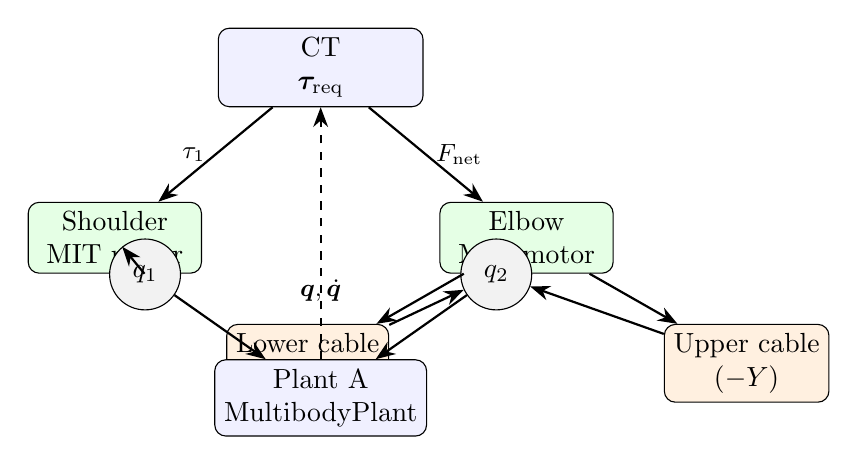
\begin{tikzpicture}[
    node distance=1.1cm and 1.4cm,
    block/.style={draw, rounded corners, minimum width=2.6cm, minimum height=0.9cm,
                  align=center, fill=blue!6},
    motor/.style={draw, rounded corners, minimum width=2.2cm, minimum height=0.8cm,
                  align=center, fill=green!10},
    cable/.style={draw, rounded corners, minimum width=2.0cm, minimum height=0.7cm,
                  align=center, fill=orange!12},
    joint/.style={circle, draw, minimum size=0.9cm, fill=gray!10},
    arr/.style={-{Stealth[length=2.5mm]}, thick},
]

\node[block] (ct) {CT\\$\btau_{\mathrm{req}}$};
\node[motor, below left=1.2cm and 0.2cm of ct] (m1) {Shoulder\\MIT motor};
\node[motor, below right=1.2cm and 0.2cm of ct] (m2) {Elbow\\MIT motor};
\node[cable, below left=0.9cm of m2] (clo) {Lower cable\\$(+Y)$};
\node[cable, below right=0.9cm of m2] (cup) {Upper cable\\$(-Y)$};
\node[joint, below left=1.8cm and 0.6cm of ct] (j1) {$q_1$};
\node[joint, below right=1.8cm and 0.6cm of ct] (j2) {$q_2$};
\node[block, below=3.2cm of ct] (pa) {Plant A\\MultibodyPlant};

\draw[arr] (ct) -- node[left, font=\small]{$\tau_1$} (m1);
\draw[arr] (ct) -- node[right, font=\small]{$F_{\mathrm{net}}$} (m2);
\draw[arr] (m1) -- (j1);
\draw[arr] (m2) -- (clo);
\draw[arr] (m2) -- (cup);
\draw[arr] (clo) -- (j2);
\draw[arr] (cup) -- (j2);
\draw[arr] (j1) -- (pa);
\draw[arr] (j2) -- (pa);
\draw[arr, dashed] (pa.north) -- ++(0,0.6) -| node[near start, above, font=\small]{$\bq,\bqd$} (ct);

\end{tikzpicture}
\caption{Hardware topology: shoulder direct-drive; elbow one motor, two antagonistic cables.}
\label{fig:hardware}
\end{figure}

% ============================================================================
\section{Repository File Map}
% ============================================================================

\begin{longtable}{@{}p{0.38\linewidth}p{0.55\linewidth}@{}}
\toprule
\textbf{Path} & \textbf{Role} \\
\midrule
\endhead
\texttt{script\_mhp\_manipulator\_cable\_framework\_pydrake.py}
  & CLI entry --- full Plant~A cable stack \\
\texttt{script\_mhp\_manipulator\_ct\_pydrake.py}
  & CLI entry --- CT-only (ideal actuators) \\
\texttt{cable/simulation\_mhp\_cable\_framework.py}
  & Drake diagram build, sim loop, logging, plots \\
\texttt{cable/simulation\_mhp\_ct.py}
  & CT-only Drake diagram + cable viz overlay \\
\texttt{controller/mhp\_ct\_controller.py}
  & Alias to \texttt{ComputedTorqueController} \\
\texttt{controller/controller.py}
  & Core CT: IK, Jacobian FF, inverse dynamics \\
\texttt{controller/mhp\_cable\_framework.py}
  & \texttt{MHPCableFramework} LeafSystem \\
\texttt{controller/cable\_wrench\_mhp.py}
  & $\btau \to F_{\mathrm{net}} \to T_{\mathrm{lower}}/T_{\mathrm{upper}}$ \\
\texttt{actuators/dummy\_mit\_motor.py}
  & Simulated CubeMars MIT-mode motor \\
\texttt{robots/mhp\_manipulator.py}
  & Drake wrapper for MHP URDF \\
\texttt{configs/robot/mhp\_configs.py}
  & URDF path, joint damping/stiffness \\
\texttt{cable/*\_mhp.py}
  & Analytical cable routing geometry + viz \\
\texttt{cable/test\_mhp\_cable\_routing\_actual\_viz.py}
  & Interactive Meshcat / Matplotlib routing demo \\
\texttt{cable/test\_elbow\_ff\_from\_cable.py}
  & Unit tests for elbow $\tau_{\mathrm{ff}}$ modes \\
\bottomrule
\end{longtable}

URDF:
\texttt{model\_using\_onshape\_to\_robot/manipulator\_hybrid\_planar\_fusion/\\
manipulator\_hybrid\_planar\_fusion\_obj.urdf}.

% ============================================================================
\section{General Architecture --- Block Diagrams}
% ============================================================================

\subsection{Plant A cable framework (closed loop)}

\begin{figure}[H]
\centering
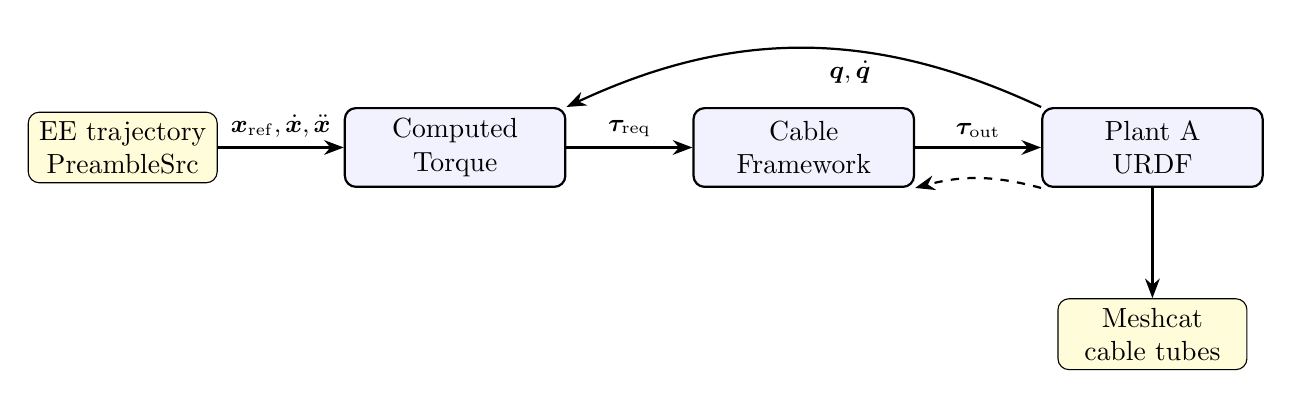
\begin{tikzpicture}[
    node distance=0.9cm and 1.2cm,
    sys/.style={draw, thick, rounded corners, minimum height=1.0cm,
                minimum width=2.8cm, align=center, fill=blue!5},
    src/.style={draw, rounded corners, minimum height=0.8cm,
                minimum width=2.4cm, align=center, fill=yellow!15},
    arr/.style={-{Stealth[length=2.5mm]}, thick},
]

\node[src] (traj) {EE trajectory\\PreambleSrc};
\node[sys, right=1.6cm of traj] (ct) {Computed\\Torque};
\node[sys, right=1.6cm of ct] (cfw) {Cable\\Framework};
\node[sys, right=1.6cm of cfw] (pa) {Plant A\\URDF};
\node[src, below=1.4cm of pa] (viz) {Meshcat\\cable tubes};

\draw[arr] (traj) -- node[above, font=\small]{$\bx_{\mathrm{ref}},\dot\bx,\ddot\bx$} (ct);
\draw[arr] (ct) -- node[above, font=\small]{$\btau_{\mathrm{req}}$} (cfw);
\draw[arr] (cfw) -- node[above, font=\small]{$\btau_{\mathrm{out}}$} (pa);
\draw[arr] (pa.north west) to[bend right=25]
    node[below, font=\small, pos=0.4]{$\bq,\bqd$} (ct.north east);
\draw[arr] (pa.south) -- (viz);
\draw[arr, dashed] (pa.south west) to[bend right=15] (cfw.south east);

\end{tikzpicture}
\caption{Drake closed-loop diagram for \texttt{simulation\_mhp\_cable\_framework.py}.}
\label{fig:closedloop}
\end{figure}

\subsection{CT-only stack (simplified)}

\begin{figure}[H]
\centering
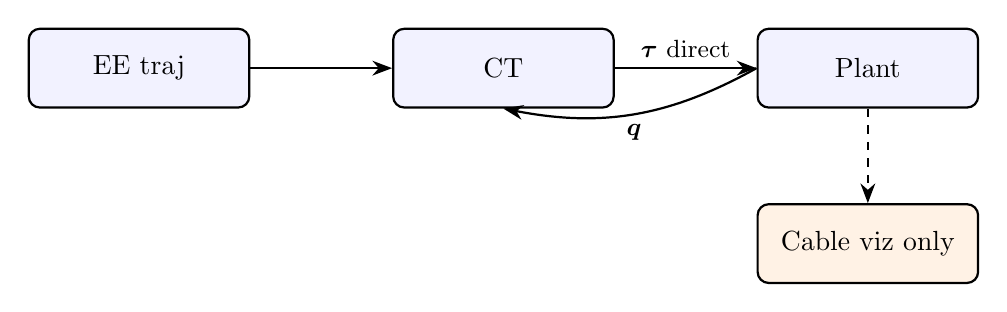
\begin{tikzpicture}[
    node distance=1.2cm,
    sys/.style={draw, thick, rounded corners, minimum height=1.0cm,
                minimum width=2.8cm, align=center, fill=blue!5},
    arr/.style={-{Stealth[length=2.5mm]}, thick},
]
\node[sys] (traj) {EE traj};
\node[sys, right=1.8cm of traj] (ct) {CT};
\node[sys, right=1.8cm of ct] (pa) {Plant};
\node[sys, below=1.2cm of pa, fill=orange!10] (viz) {Cable viz only};

\draw[arr] (traj) -- (ct);
\draw[arr] (ct) -- node[above, font=\small]{$\btau$ direct} (pa);
\draw[arr, dashed] (pa) -- (viz);
\draw[arr] (pa.west) to[bend left=20] node[below, font=\small]{$\bq$} (ct.south);
\end{tikzpicture}
\caption{CT-only: torques bypass the cable/MIT layer. Cables are visualization only.}
\label{fig:ctonly}
\end{figure}

% ============================================================================
\section{Control Equations}
% ============================================================================

\subsection{Layer 1 --- Computed torque}

Given end-effector reference $(\bx_{\mathrm{ref}}, \dot\bx_{\mathrm{ref}}, \ddot\bx_{\mathrm{ref}})$:

\begin{align}
  \bq_{\mathrm{des}} &= \mathrm{IK}(\bx_{\mathrm{ref}}) \\
  \dot\bq_{\mathrm{ref}} &= \bJ^{-1}\dot\bx_{\mathrm{ref}}, \quad
  \ddot\bq_{\mathrm{ref}} = \bJ^{-1}(\ddot\bx_{\mathrm{ref}} - \dot\bJ\dot\bq) \\
  \ba_{\mathrm{des}} &= \ddot\bq_{\mathrm{ref}} + \mathbf{K}_p(\bq_{\mathrm{des}}-\bq)
                      + \mathbf{K}_d(\dot\bq_{\mathrm{ref}}-\bqd) \\
  \btau_{\mathrm{req}} &= \bM(\bq)\,\ba_{\mathrm{des}} + \bh(\bq,\bqd)
\end{align}

Default gains: $K_{p,i}=400\;\mathrm{s}^{-2}$, $K_{d,i}=40\;\mathrm{s}^{-1}$,
$\tau_{\max}=10\;\mathrm{Nm}$.

\subsection{Layer 2 --- Cable wrench map}

From \texttt{controller/cable\_wrench\_mhp.py}:

\begin{resultbox}
\[
  F_{\mathrm{net}} = \frac{\tau_{2,\mathrm{req}}}{r_p}, \qquad
  T_{\mathrm{lower}} = \max(F_{\mathrm{net}}, 0), \qquad
  T_{\mathrm{upper}} = \max(-F_{\mathrm{net}}, 0)
\]
\[
  \mathbf{W}_{\mathrm{eff}} =
  \begin{bmatrix} 1 & 0 \\ 0 & r_p \end{bmatrix}, \qquad
  \begin{bmatrix}\tau_1 \\ \tau_2\end{bmatrix}
  \approx \mathbf{W}_{\mathrm{eff}}
  \begin{bmatrix}\tau_{m1} \\ F_{\mathrm{net}}\end{bmatrix}
\]
\end{resultbox}

\subsection{Optional tension inner loop}

When \texttt{--tension-kp} $K_F > 0$:
\[
  F_{\mathrm{meas}} = T_{\mathrm{lo,meas}} - T_{\mathrm{up,meas}}, \qquad
  F_{\mathrm{cmd}} = F_{\mathrm{net}} + K_F\,(F_{\mathrm{net}} - F_{\mathrm{meas}})
\]
Then re-split: $T_{\mathrm{lower,cmd}}=\max(F_{\mathrm{cmd}},0)$,
$T_{\mathrm{upper,cmd}}=\max(-F_{\mathrm{cmd}},0)$.

\subsection{Elbow MIT feed-forward modes}

\begin{table}[H]
\centering
\caption{Elbow $\tau_{\mathrm{ff},2}$ sources (\texttt{--elbow-ff-from-cable}, default ON)}
\begin{tabular}{@{}ll@{}}
\toprule
\textbf{Mode} & \textbf{Elbow MIT feed-forward} \\
\midrule
Default (\texttt{--elbow-ff-from-cable}) & $\tau_{\mathrm{ff},2} = r_p\,F_{\mathrm{cmd}}$ \\
Legacy (\texttt{--no-elbow-ff-from-cable}) & $\tau_{\mathrm{ff},2} = \tau_{2,\mathrm{req}}$ (raw CT) \\
\bottomrule
\end{tabular}
\end{table}

\subsection{Layer 3 --- MIT motor law}

From \texttt{actuators/dummy\_mit\_motor.py}:
\[
  \tau_m = K_p\,(p_{\mathrm{des}}-p) + K_d\,(v_{\mathrm{des}}-v) + \tau_{\mathrm{ff}}
\]
Algebraic mode (default): $\tau_{\mathrm{out}}=\tau_m$ immediately.
Optional rotor dynamics: $J_m\ddot\theta_m = \tau_m - b_m\dot\theta_m$.

% ============================================================================
\section{In-Depth Signal Flow (One Timestep)}
% ============================================================================

\begin{figure}[H]
\centering
\resizebox{\linewidth}{!}{%
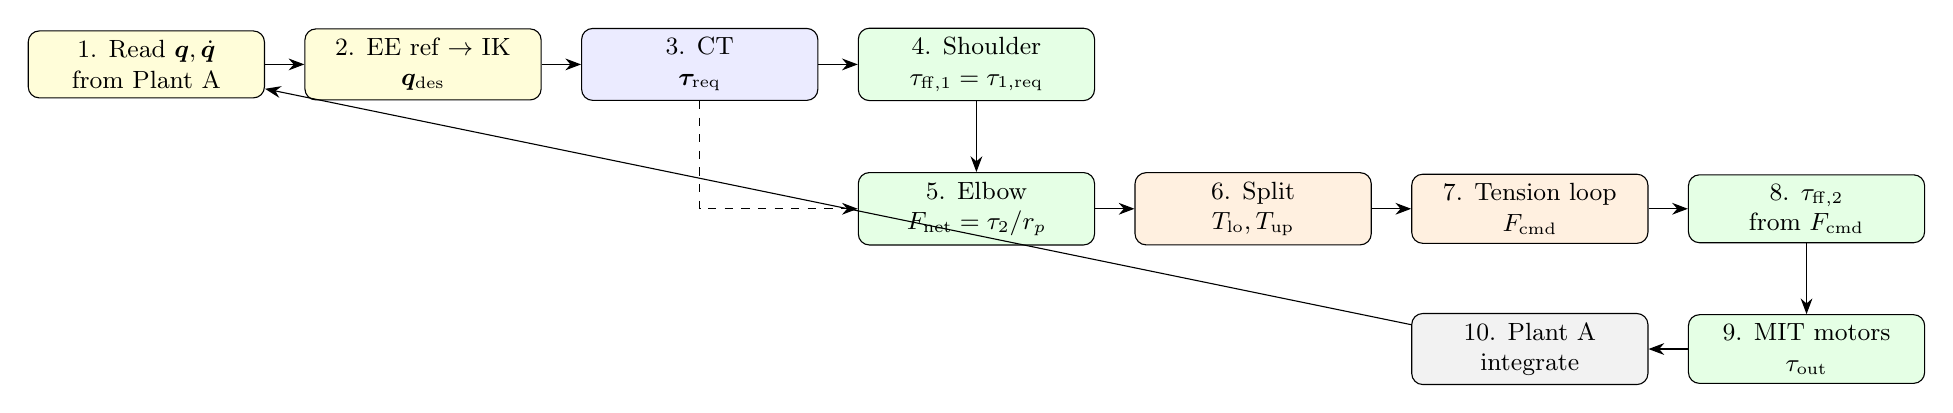
\begin{tikzpicture}[
    flowstep/.style={draw, rounded corners, minimum width=3.0cm, minimum height=0.85cm,
                 align=center, font=\small},
    arr/.style={-{Stealth[length=2mm]}},
    lbl/.style={font=\scriptsize, fill=white, inner sep=1pt},
]

\node[flowstep, fill=yellow!15] (s1) {1. Read $\bq,\bqd$\\from Plant A};
\node[flowstep, fill=yellow!15, right=0.5cm of s1] (s2) {2. EE ref $\to$ IK\\$\bq_{\mathrm{des}}$};
\node[flowstep, fill=blue!8, right=0.5cm of s2] (s3) {3. CT\\$\btau_{\mathrm{req}}$};
\node[flowstep, fill=green!10, right=0.5cm of s3] (s4) {4. Shoulder\\$\tau_{\mathrm{ff},1}=\tau_{1,\mathrm{req}}$};
\node[flowstep, fill=green!10, below=0.9cm of s4] (s5) {5. Elbow\\$F_{\mathrm{net}}=\tau_2/r_p$};
\node[flowstep, fill=orange!12, right=0.5cm of s5] (s6) {6. Split\\$T_{\mathrm{lo}},T_{\mathrm{up}}$};
\node[flowstep, fill=orange!12, right=0.5cm of s6] (s7) {7. Tension loop\\$F_{\mathrm{cmd}}$};
\node[flowstep, fill=green!10, right=0.5cm of s7] (s8) {8. $\tau_{\mathrm{ff},2}$\\from $F_{\mathrm{cmd}}$};
\node[flowstep, fill=green!10, below=0.9cm of s8] (s9) {9. MIT motors\\$\tau_{\mathrm{out}}$};
\node[flowstep, fill=gray!10, left=0.5cm of s9] (s10) {10. Plant A\\integrate};

\foreach \a/\b in {s1/s2,s2/s3,s3/s4,s4/s5,s5/s6,s6/s7,s7/s8,s8/s9,s9/s10,s10/s1}{
  \draw[arr] (\a) -- (\b);
}
\draw[arr, dashed] (s3.south) |- (s5.west);

\end{tikzpicture}%
}
\caption{Per-timestep control cycle inside \texttt{MHPCableFramework.\_solve()} (500\,Hz).}
\label{fig:timestep}
\end{figure}

% ============================================================================
\section{Full State Diagram}
% ============================================================================

The diagram below shows \emph{all signals and state variables} carried through
one simulation tick.  Plant state closes the loop; cable routing geometry is
a parallel visualization path (not in the force loop).

\begin{figure}[H]
\centering
\resizebox{\linewidth}{!}{%
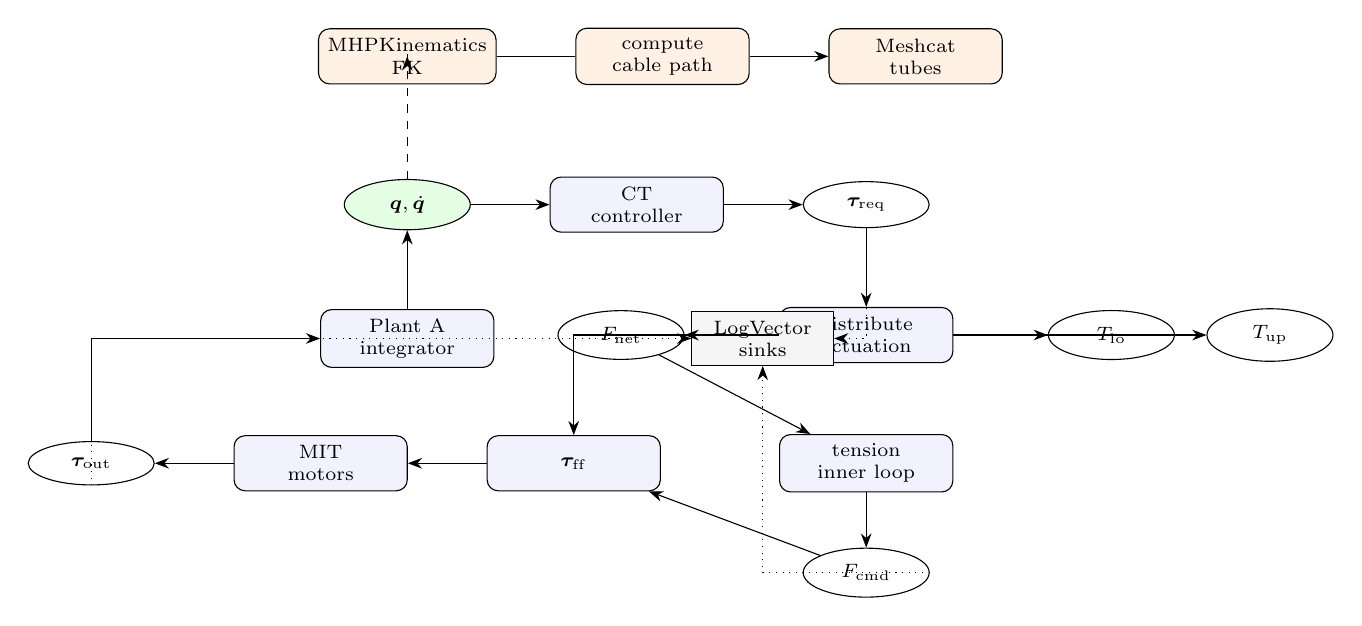
\begin{tikzpicture}[
    font=\scriptsize,
    var/.style={ellipse, draw, minimum width=1.6cm, minimum height=0.55cm, align=center},
    proc/.style={rectangle, draw, rounded corners, minimum width=2.2cm,
                  minimum height=0.7cm, align=center, fill=blue!5},
    store/.style={rectangle, draw, minimum width=1.8cm, minimum height=0.55cm,
                  align=center, fill=gray!8},
    arr/.style={-{Stealth[length=1.8mm]}},
]

% Plant state
\node[var, fill=green!10] (q) {$\bq,\bqd$};
\node[proc, right=1.0cm of q] (ct) {CT\\controller};
\node[var, right=1.0cm of ct] (taureq) {$\btau_{\mathrm{req}}$};

% Cable framework internals
\node[proc, below=1.0cm of taureq] (dist) {distribute\\actuation};
\node[var, left=1.2cm of dist] (fnet) {$F_{\mathrm{net}}$};
\node[var, right=1.2cm of dist] (tlo) {$T_{\mathrm{lo}}$};
\node[var, right=0.4cm of tlo] (tup) {$T_{\mathrm{up}}$};

\node[proc, below=0.9cm of dist] (tloop) {tension\\inner loop};
\node[var, below=0.7cm of tloop] (fcmd) {$F_{\mathrm{cmd}}$};

\node[proc, left=1.5cm of tloop] (tff) {$\btau_{\mathrm{ff}}$};
\node[proc, left=1.0cm of tff] (mit) {MIT\\motors};
\node[var, left=1.0cm of mit] (tauout) {$\btau_{\mathrm{out}}$};

\node[proc, below=1.0cm of q] (plant) {Plant A\\integrator};
\node[store, right=2.5cm of plant] (logs) {LogVector\\sinks};

% Viz branch
\node[proc, above=1.2cm of q, fill=orange!10] (fk) {MHPKinematics\\FK};
\node[proc, right=1.0cm of fk, fill=orange!10] (path) {compute\\cable path};
\node[proc, right=1.0cm of path, fill=orange!10] (mesh) {Meshcat\\tubes};

% Connections
\draw[arr] (q) -- (ct);
\draw[arr] (ct) -- (taureq);
\draw[arr] (taureq) -- (dist);
\draw[arr] (dist) -- (fnet);
\draw[arr] (dist) -- (tlo);
\draw[arr] (dist) -- (tup);
\draw[arr] (fnet) -- (tloop);
\draw[arr] (tloop) -- (fcmd);
\draw[arr] (fcmd) -- (tff);
\draw[arr] (dist.west) -| (tff.north);
\draw[arr] (tff) -- (mit);
\draw[arr] (mit) -- (tauout);
\draw[arr] (tauout) |- (plant);
\draw[arr] (plant) -- (q);
\draw[arr, dashed] (q) |- (fk);
\draw[arr] (fk) -- (path) -- (mesh);

% Log taps
\draw[arr, dotted] (taureq.south) |- (logs);
\draw[arr, dotted] (tauout.south) |- (logs);
\draw[arr, dotted] (fcmd.east) -| (logs);

\end{tikzpicture}%
}
\caption{Full state/signal diagram: control loop (solid) vs.\ cable viz branch (orange, dashed).}
\label{fig:fulldiag}
\end{figure}

\textbf{Logged signals} (cable framework run):
\begin{itemize}[noitemsep]
  \item \texttt{log\_state} --- full multibody state
  \item \texttt{log\_tau\_req} --- CT raw torques
  \item \texttt{log\_tau\_out} --- MIT output torques
  \item \texttt{log\_tensions}, \texttt{log\_t\_meas} --- commanded / measured cable tensions
  \item \texttt{log\_tau\_ff} --- MIT feed-forward $[\tau_{\mathrm{ff},1}, \tau_{\mathrm{ff},2}]$
  \item \texttt{log\_cable\_cmd} --- $[F_{\mathrm{net}}, F_{\mathrm{cmd}}, \tau_{\mathrm{ff},2}]$
  \item \texttt{log\_qdes}, \texttt{log\_ref}, \texttt{log\_diag}
\end{itemize}

Plots saved to \texttt{plots/mhp\_cable\_fw\_\{traj\}\_\{timestamp\}.png}.

% ============================================================================
\section{Script Reference and CLI Examples}
% ============================================================================

\subsection{\texttt{script\_mhp\_manipulator\_cable\_framework\_pydrake.py}}

\begin{table}[H]
\centering
\caption{Cable framework CLI arguments (defaults)}
\small
\begin{tabular}{@{}lll@{}}
\toprule
\textbf{Group} & \textbf{Argument} & \textbf{Default} \\
\midrule
CT & \texttt{--ct-kp}, \texttt{--ct-kd} & $[400,400]$, $[40,40]$ \\
CT & \texttt{--ct-tau-max} & $10\;\mathrm{Nm}$ \\
MIT & \texttt{--mit-kp}, \texttt{--mit-kd} & $[30,15]$, $[1.5,0.5]$ \\
MIT & \texttt{--mit-dynamics} & off \\
Tension & \texttt{--tension-kp} & $0.5$ \\
Tension & \texttt{--tension-noise} & $0\;\mathrm{N}$ \\
Elbow FF & \texttt{--elbow-ff-from-cable} & \textbf{ON} \\
Sim & \texttt{--duration}, \texttt{--move-duration} & $10\;\mathrm{s}$, $3\;\mathrm{s}$ \\
Traj & \texttt{--traj-type} & \texttt{rect} \\
Viz & \texttt{--no-meshcat}, \texttt{--no-show} & Meshcat on, plots show \\
\bottomrule
\end{tabular}
\end{table}

\textbf{Examples:}
\begin{lstlisting}[style=python, caption={Cable framework --- common invocations}]
# Default: cable-consistent elbow ff, Meshcat + plots
python script_mhp_manipulator_cable_framework_pydrake.py

# Headless short run
python script_mhp_manipulator_cable_framework_pydrake.py \
    --no-meshcat --no-show --duration 4 --move-duration 0

# Legacy: elbow ff tracks raw CT torque
python script_mhp_manipulator_cable_framework_pydrake.py \
    --no-elbow-ff-from-cable

# Circle trajectory with stronger tension loop
python script_mhp_manipulator_cable_framework_pydrake.py \
    --traj-type circle --tension-kp 1.0 --duration 8

# Rotor dynamics on MIT motors
python script_mhp_manipulator_cable_framework_pydrake.py \
    --mit-dynamics --mit-kp 40 20 --mit-kd 2 1
\end{lstlisting}

\subsection{\texttt{script\_mhp\_manipulator\_ct\_pydrake.py}}

Same CT, simulation, robot, and trajectory groups --- \textbf{no} MIT/tension/elbow-ff
arguments (cables are viz-only).

\begin{lstlisting}[style=python, caption={CT-only examples}]
python script_mhp_manipulator_ct_pydrake.py
python script_mhp_manipulator_ct_pydrake.py --traj-type circle --duration 8
python script_mhp_manipulator_ct_pydrake.py --ct-kp 400 400 --ct-kd 40 40 --no-show
\end{lstlisting}

\subsection{\texttt{cable/test\_mhp\_cable\_routing\_actual\_viz.py}}

\begin{lstlisting}[style=python, caption={Cable routing visualization}]
python cable/test_mhp_cable_routing_actual_viz.py
python cable/test_mhp_cable_routing_actual_viz.py --q1 30 --q2 -20
python cable/test_mhp_cable_routing_actual_viz.py --no-matplotlib
\end{lstlisting}

Interactive Meshcat loop: enter \texttt{q1 q2} in degrees to update pose.

% ============================================================================
\section{Key Code Snippets}
% ============================================================================

\subsection{Drake diagram wiring (cable framework)}

\begin{lstlisting}[style=python, caption={cable/simulation\_mhp\_cable\_framework.py (connections)}]
builder.Connect(ct.GetOutputPort("actuation"), cable_fw.GetInputPort("tau_req"))
builder.Connect(plant_a.get_state_output_port(), cable_fw.GetInputPort("plant_state"))
builder.Connect(cable_fw.GetOutputPort("actuation"), plant_a.get_actuation_input_port())
\end{lstlisting}

\subsection{Antagonistic tension split}

\begin{lstlisting}[style=python, caption={controller/cable\_wrench\_mhp.py}]
F_net = float(tau_req[1] / r_p)
T_lower = max(F_net, 0.0)    # +Y side
T_upper = max(-F_net, 0.0)   # -Y side
tau_elbow_ff = float(tau_req[1])   # default CT path
\end{lstlisting}

\subsection{Elbow ff from cable command}

\begin{lstlisting}[style=python, caption={controller/mhp\_cable\_framework.py (\_solve)}]
if self._elbow_ff_from_cable:
    tau_elbow_ff = elbow_torque_from_cable_command(F_cmd, self._wrench_cfg.r_elbow)
else:
    tau_elbow_ff = dist["tau_elbow_ff"]

tau_ff = tensions_to_mit_feedforward(dist["tau_shoulder_ff"], tau_elbow_ff)
\end{lstlisting}

\subsection{MIT motor step}

\begin{lstlisting}[style=python, caption={actuators/dummy\_mit\_motor.py}]
tau_m = kp * (p_des - p) + kd * (v_des - v) + tau_ff
\end{lstlisting}

\subsection{CT-only direct actuation}

\begin{lstlisting}[style=python, caption={cable/simulation\_mhp\_ct.py}]
builder.Connect(ct.GetOutputPort("actuation"), plant.get_actuation_input_port())
\end{lstlisting}

% ============================================================================
\section{Cable Routing Modules (\texttt{cable/*\_mhp.py})}
% ============================================================================

Routing geometry is \textbf{decoupled} from the control loop.  The sim updates
Meshcat cable tubes from $(q_1,q_2)$ via analytical FK --- no Drake cable force elements.

\begin{figure}[H]
\centering
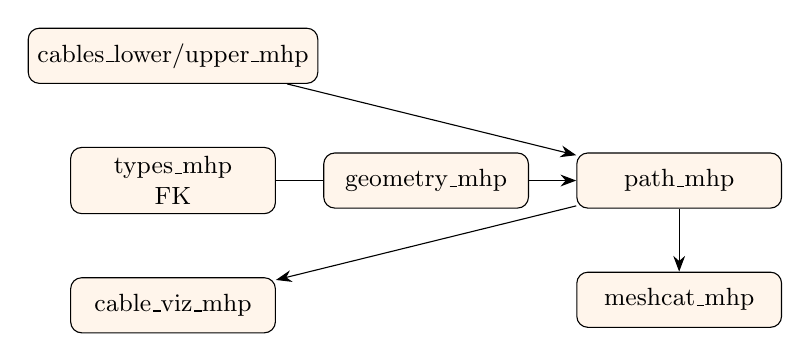
\begin{tikzpicture}[
    node distance=0.8cm,
    mod/.style={draw, rounded corners, minimum width=2.6cm, minimum height=0.7cm,
                align=center, font=\small, fill=orange!8},
    arr/.style={-{Stealth[length=2mm]}},
]
\node[mod] (types) {types\_mhp\\FK};
\node[mod, right=0.6cm of types] (geom) {geometry\_mhp};
\node[mod, right=0.6cm of geom] (path) {path\_mhp};
\node[mod, below=0.8cm of path] (mesh) {meshcat\_mhp};
\node[mod, below=0.8cm of types] (viz) {cable\_viz\_mhp};
\node[mod, above=0.8cm of types] (cfg) {cables\_lower/upper\_mhp};

\draw[arr] (cfg) -- (path);
\draw[arr] (types) -- (geom) -- (path);
\draw[arr] (path) -- (mesh);
\draw[arr] (path) -- (viz);
\end{tikzpicture}
\caption{Cable routing module pipeline (visualization only).}
\end{figure}

% ============================================================================
\section{CT-Only vs.\ Cable Framework}
% ============================================================================

\begin{table}[H]
\centering
\caption{Comparison of the two MHP simulation stacks}
\begin{tabular}{@{}p{0.22\linewidth}p{0.35\linewidth}p{0.35\linewidth}@{}}
\toprule
\textbf{Aspect} & \textbf{CT-only} & \textbf{Cable framework} \\
\midrule
Control chain & Traj $\to$ CT $\to$ plant & Traj $\to$ CT $\to$ framework $\to$ plant \\
Shoulder actuation & Ideal $\tau_1$ & Direct-drive MIT \\
Elbow actuation & Ideal $\tau_2$ & One motor + antagonistic cables \\
Cable in force loop & No & Yes ($F_{\mathrm{net}}$, tension loop) \\
Extra CLI & --- & \texttt{--mit-*}, \texttt{--tension-*}, \texttt{--elbow-ff-*} \\
Log channels & 5 & 10 \\
Use case & Trajectory / CT tuning & Sim-to-real / hardware path \\
\bottomrule
\end{tabular}
\end{table}

\begin{warnbox}[title={Not the legacy cup/exo stack}]
The cup-manipulator scripts (\texttt{script\_cup\_manipulator\_pendulam\_tendon\_with\_exo\_pydrake.py},
SEA spring models, exosuit co-contraction) are \textbf{digital-twin only} and do not
represent the real MHP hardware.  Do not wire \texttt{SEACableActuator} or high-$k_s$
spring hacks for MHP.
\end{warnbox}

% ============================================================================
\section{Real Hardware Path (Future)}
% ============================================================================

The dummy MIT motors map directly to CubeMars drivers:
\begin{itemize}[noitemsep]
  \item \texttt{drivers/cubemars/motor.py} --- CAN MIT mode
  \item Shoulder: send $\tau_{\mathrm{ff},1}$ as MIT feed-forward
  \item Elbow: send $\tau_{\mathrm{ff},2}=r_p F_{\mathrm{cmd}}$; load cells on taut strand
        close the tension inner loop at the same rate as simulation ($500\;\mathrm{Hz}$ target)
\end{itemize}

% ============================================================================
\section{Quick Reference Card}
% ============================================================================

\begin{resultbox}
\textbf{One-line summary:}
CT plans $[\tau_1,\tau_2]$; the cable framework sends $\tau_1$ straight to the
shoulder MIT motor and maps $\tau_2$ to antagonistic cable tensions via
$F_{\mathrm{net}}=\tau_2/r_p$; one elbow motor drives both cables (one taut);
Plant~A integrates $\btau_{\mathrm{out}}$ and feeds $\bq,\bqd$ back to CT.
\end{resultbox}

\vfill
\hrule
\small
\noindent
Source repo: \texttt{Isaac\_sim\_robotics}.
Compile: \texttt{pdflatex mhp\_manipulator\_implementation.tex} (run twice for TOC).

\end{document}
